% chapters/hbm.tex
%
% Copyright 2022 Alexander Lyttle.
%
% This work may be distributed and/or modified under the conditions of the
% LaTeX Project Public License (LPPL) version 1.3 or later.
%
% The latest version of this license is in
% https://www.latex-project.org/lppl.txt and version 1.3 or later is part of
% all distributions of LaTeX version 2005/12/01 or later.
%
%
\chapter{Hierarchical Bayesian Models}\label{chap:hbm}

\textit{In this chapter, I introduce the concept of a hierarchical Bayesian model in the context of determining stellar parameters. Using a simplified analogy for measuring distances to stars in an open cluster, I demonstrate the advantages and usage of a hierarchical model in Section \ref{sec:hbm-dist}. Finally, I identify parameters which could be treated hierarchically when modelling the physical properties of stars, preparing the reader for Chapter \ref{chap:hmd}.}

\section{Introduction}

When modelling a single star, we can use a variant of Bayes' theorem (Equation \ref{eq:bayes}) to estimate the posterior probability of its parameters. We choose priors to represent our current knowledge. For example, if we observe a star in the Milky Way at random, we expect its mass to belong to an Initial Mass Function \citep[IMF; e.g.][]{Chabrier2003} without other prior knowledge. In fact, an IMF prior is an input option for BASTA \citep{AguirreBorsen-Koch.Rorsted.ea2022}. Other prior assumptions include a helium enrichment law which determines the star's initial helium abundance from its metallicity, or that its age must not be older than the universe.

Let us consider modelling a large population of stars simultaneously. For example, we may want to create a catalogue of stellar parameters to use in exoplanet and galactic research. We could treat the parameters for each star independently, repeating the modelling procedure for each star in the sample. However, we know that stars belong to population distributions like the IMF. In some cases, these population distributions are not well understood and assuming one exactly can introduce bias into our model. Instead, it could be better to let the data inform such population priors.

Hierarchical (or multi-level) Bayesian models parametrise population-level prior distributions on individual stellar parameters. These population-parameters (\emph{hyperparameters}) which govern the population must themselves have prior distributions as per the Bayesian formalisation. The hierarchical aspect comes from the distinction between hyperparameters which take one value across a population and those which vary from star-to-star. In the next section, we go through a simple example hierarchical model. Then, we discuss a few parameters which could be given the hierarchical treatment in Section \ref{sec:hbm-phys}.

\section[Stellar Distances]{Stellar Distances in an Open Cluster Analogue}\label{sec:hbm-dist}

\newcommand{\appmag}{\ensuremath{\mathrm{v}}}
\newcommand{\absmag}{\ensuremath{\mathrm{V}}}

In this section, we use the example of measuring distances to stars in an open cluster to demonstrate a hierarchical Bayesian model (HBM). This example is loosely based on the work of \citet{Leistedt.Hogg2017}, which presents a hierarchical model of the colour-magnitude diagram to improve distances from \emph{Gaia} \citep{GaiaCollaboration.Prusti.ea2016}. However, instead of considering the population distributions over magnitude and colour, we build a hierarchy over the stellar distances.

We created a dataset analogous to an open cluster of \(N_\mathrm{stars}=20\) stars. We gave each \(i\)-th star a dimensionless distance (\(d_i\)) from the observer drawn randomly from a normal distribution with a mean of 10 and standard deviation of 0.1. Then, we converted these to dimensionless parallax using the relation \(\varpi = 1/d\). We also gave each star an absolute visual magnitude (\(\absmag_i\)) drawn randomly from a standard normal distribution. To get a quantity proportional to apparent magnitude (\(\appmag_i\)) for each star, we used the relation \(\appmag_i = \absmag_i + 5 \log_{10} d_i\). For the purpose of this example, we ignored additional real-world effects such as extinction and reddening.

% \begin{table}[tb]
%     \centering
%     \caption{Simulated dimensionless distance, magnitudes and parallax for \(N_\mathrm{stars}=20\) belonging to an open cluster analogue.}
%     \label{tab:hbm-data}
%     \begin{tabular}{r|rrrr|rr}
\toprule
 & $d_\mathrm{true}$ & $\mathrm{V_{true}}$ & $\varpi_\mathrm{true}$ & $\mathrm{v_{true}}$ & $\varpi_\mathrm{obs}$ & $\mathrm{v_{obs}}$ \\
Star &  &  &  &  &  &  \\
\midrule
0 & 9.9590 & -1.2758 & 0.10041 & 3.7153 & 0.09439 & 3.5628 \\
1 & 10.1730 & 0.3098 & 0.09830 & 5.3471 & 0.09202 & 5.3523 \\
2 & 10.1205 & -0.6844 & 0.09881 & 4.3416 & 0.10593 & 4.3648 \\
3 & 9.8957 & 0.7540 & 0.10105 & 5.7312 & 0.11552 & 5.9872 \\
4 & 10.1023 & 0.7008 & 0.09899 & 5.7229 & 0.09636 & 5.6452 \\
5 & 10.0334 & 0.2487 & 0.09967 & 5.2559 & 0.09678 & 5.2154 \\
6 & 9.9949 & 0.5171 & 0.10005 & 5.5160 & 0.09456 & 5.5110 \\
7 & 10.0877 & -3.2752 & 0.09913 & 1.7437 & 0.09919 & 1.7812 \\
8 & 10.2116 & -0.4053 & 0.09793 & 4.6402 & 0.08759 & 4.6816 \\
9 & 9.8786 & -0.4657 & 0.10123 & 4.5078 & 0.10183 & 4.5158 \\
10 & 10.0208 & -1.0131 & 0.09979 & 3.9914 & 0.12611 & 4.0295 \\
11 & 9.9049 & 1.2571 & 0.10096 & 6.2363 & 0.08160 & 6.4150 \\
12 & 9.8902 & -1.8509 & 0.10111 & 3.1251 & 0.10719 & 3.1597 \\
13 & 9.8521 & 0.8966 & 0.10150 & 5.8642 & 0.11467 & 5.8742 \\
14 & 9.9199 & 0.5401 & 0.10081 & 5.5226 & 0.09802 & 5.3892 \\
15 & 10.0848 & -0.6031 & 0.09916 & 4.4152 & 0.10617 & 4.3134 \\
16 & 9.9546 & 0.7726 & 0.10046 & 5.7627 & 0.09763 & 5.8150 \\
17 & 10.0821 & -1.2505 & 0.09919 & 3.7672 & 0.11883 & 3.6586 \\
18 & 10.0387 & -0.4488 & 0.09961 & 4.5596 & 0.07481 & 4.6057 \\
19 & 10.0174 & 1.0101 & 0.09983 & 6.0139 & 0.09255 & 5.9360 \\
\bottomrule
\end{tabular}

% \end{table}

We simulated noisy observations of \(\varpi_i\) and \(\appmag_i\) by randomly drawing from a normal distribution centred on their true values with standard deviations of \(\sigma_{\appmag,i} = 0.1\) and \(\sigma_{\varpi,i} = 0.01\) respectively. 
% We repeated this for \(N_\mathrm{stars}=20\) stars and present the true values and observables in Table \ref{tab:hbm-data}. 
For real-world context, the uncertainties on \(\varpi\) from \emph{Gaia} \citep{GaiaCollaboration.Prusti.ea2016} Data Release 3 \citep[][]{GaiaCollaboration.Vallenari.ea2022} are approximately \SI{0.02}{\milli\aarcsec} for stars with \emph{Gaia} G-band magnitudes of less than 15. Therefore, if our choice of \(\sigma_{\varpi,i}\) was representative of \emph{Gaia} uncertainties, then the distance to our stellar cluster would be \(\sim \SI{5}{\kilo\parsec}\). An example open cluster at this distance is NGC 6791, at \SI{4}{\kilo\parsec} \citep{Brogaard.Bruntt.ea2011}. We note that by the same comparison, our chosen spread in dimensionless distances of 0.1 corresponds to an order of magnitude more than typical cluster sizes of a few parsecs. However, we chose to exaggerate the distance spread to make it easier to detect for the purpose of this example.

In Section \ref{sec:simple-model}, we describe a simple Bayesian model for determining distances and absolute magnitudes of stars in the cluster. Then, we define the HBM in Section \ref{sec:hbm-model} which incorporates a population-level distribution over distance. We outline our method for inferring model parameters in Section \ref{sec:hbm-inf} and then compare results from the models in Section \ref{sec:hbm-comp}. Finally, we explore how the HBM scales with the number of stars observed in Section \ref{sec:hbm-scale}.

\subsection{Simple Model}\label{sec:simple-model}

We started with a simple model which treats each star independently. Using Bayes' theorem, we write the posterior probability density of the model parameters, \(d_i, \absmag_i\) given the observed parameters \(\varpi_i, \appmag_i\) as,
%
\begin{equation}
    p(d_i, \absmag_i \mid \varpi_i, \appmag_i) \propto p(\varpi_i, \appmag_i \mid d_i, \absmag_i) \, p(d_i, \absmag_i).
\end{equation}
%
The likelihood is given by \(p(\varpi_i, \appmag_i \mid d_i, \absmag_i)\) and the prior probability of the parameters is \(p(d_i, \absmag_i)\).

We modelled the likelihood as the product of normal distributions, assuming \(\varpi_i\) and \(\appmag_i\) were observed independently,
%
\begin{equation}
    p(\varpi_i, \appmag_i \mid d_i, \absmag_i) = \mathcal{N}(\varpi_i \mid d_i^{\,-1}, \sigma_{\varpi, i}^2) \, \mathcal{N}(\appmag_i \mid \absmag_i + 5\log_{10}d_i \, , \sigma_{\appmag, i}^2),\label{eq:hbm-like}
\end{equation}
%
where \(\mathcal{N}(x \,|\, \mu, \sigma^2)\) is a normal distribution over \(x\) with a mean of \(\mu\) and variance of \(\sigma^2\).

We assumed stars in the cluster were equally likely to be between a distance of 0 and 20. Moreover, we assumed the absolute magnitudes were likely to be normally distributed centred on 0 and scaled by 10. Therefore, the prior probability of the model parameters was,
%
\begin{equation}
    p(d_i, \absmag_i) = \mathcal{U}(d_i \mid 0, 20) \, \mathcal{N}(\absmag_i \mid 0, 100),
\end{equation}
%
where \(\mathcal{U}(x \,|\, a, b)\) is a uniform distribution over \(x\) from \(a\) to \(b\). We chose wide, weakly-informative priors here because the focus of this example is on the hierarchical component introduced in the next section. However, the priors should be chosen more carefully in a real-world application.
% However, these priors are fairly unrealistic and should be adapted to represent our expectation in real-world cases. For example, the exponential prior from \citet{Bailer-Jones.Rybizki.ea2018} would me more appropriate when observing stars radially outward from the galactic disk.

\begin{figure}[tb]
    \centering
    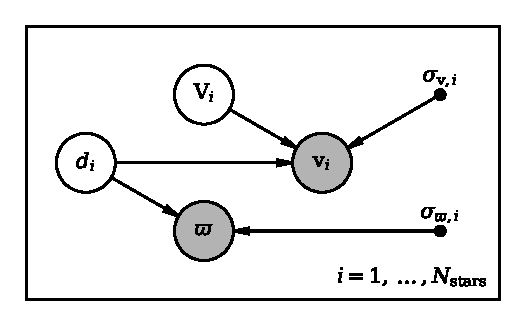
\includegraphics{figures/simple-pgm.pdf}
    \caption[Probabilistic graphical model for the simple (non-hierarchical) model]{Probabilistic graphical model for the simple (non-hierarchical) model. Parameters are given by circular nodes and connected by arrows showing the direction of dependency. Observed parameters are shaded, and fixed parameters are given by filled dots. The box represents a set of parameters belonging to the \(i\)-th star. \emph{This diagram was made using the \textsc{Python} package \texttt{daft} \citep{Foreman-Mackey.Hogg.ea2021}.}}
    \label{fig:simple-pgm}
\end{figure}

In Figure \ref{fig:simple-pgm}, we show a probabilistic graphical model of the simple model. This shows the connections between parameters in the model. There is no hierarchy in this model because each parameter exists within the box, meaning no parameters are shared between stars. However, we know that the stellar distances are correlated. For example, it is highly unlikely that one star in the cluster is at a distance of 5 and another is at a distance of 15. If we can exploit this expectation, we could improve our prior and thus improve the inference of \(d_i\) and \(\absmag_i\).

\subsection{Hierarchical Model}\label{sec:hbm-model}

In this section, we present an HBM which includes the known correlation between distances to the stars in this open cluster analogue. We assumed the stars are all members of the same open cluster. Therefore, their distances can be modelled by some tight distribution. For this example, we assumed that each distance is drawn from a normal distribution characterised by new \emph{hyperparameters} \(\mu_d\) and \(\sigma_d\),
%
\begin{equation}
    d_i \sim \mathcal{N}(\mu_d, \sigma_d^2).
\end{equation}
%
The hyperparameters are so-called because they take a single value for the population of stars. Hence, the hierarchy of the model arises as some parameters represent how individual parameters are distributed in the population.

Each stellar distance, \(d_i\), is no longer treated independently by the model. Hence, we modified the posterior probability distribution to account for this correlation,
%
\begin{equation}
    p(\mu_d, \sigma_d, \vect{d}, \vect{\absmag} \mid \vect{\varpi}, \vect{\appmag}) \propto p(\vect{\varpi}, \vect{\appmag} \mid \vect{d}, \vect{\absmag}) \, p(\vect{d} \mid \mu_d, \sigma_d) \, p(\mu_d, \sigma_d, \vect{\absmag}),
\end{equation}
%
where \(p(\vect{\varpi}, \vect{\appmag} \mid \vect{d}, \vect{\absmag})\) is the likelihood --- a product over Equation \ref{eq:hbm-like},
%
\begin{equation}
    p(\vect{\varpi}, \vect{\appmag} \mid \vect{d}, \vect{\absmag}) = \prod_{i=1}^{N_\mathrm{stars}} p(\varpi_i, \appmag_i \mid d_i, \absmag_i).
\end{equation}
%
Our posterior now depends on all stars in the population, so we used bold symbols to represent the set of individual stellar parameters. For example, \(\vect{d} \equiv d_1, \dots, d_{N_\mathrm{stars}}\).

We modelled \(d_i\) as a random variable which depends on the hyperparameters. This is why our prior became the product of a conditional distribution, \(p(\vect{d} \,|\, \mu_d, \sigma_d)\) and a prior on the remaining independent parameters, \(p(\mu_d, \sigma_d, \vect{\absmag})\). We write the conditional distribution for distance as a product of normal distributions,
%
\begin{equation}
    p(\vect{d} \mid \mu_d, \sigma_d) = \prod_{i=1}^{N_\mathrm{stars}} \mathcal{N}(d_i \mid \mu_d, \sigma_d^2),
\end{equation}
%
where the prior probability distribution for \(\mu_d\) and \(\sigma_d\) is,
%
\begin{equation}
    p(\mu_d, \sigma_d) = \mathcal{U}(\mu_d \mid 0, 20) \, \mathcal{N}(\ln\sigma_d \mid - \ln 10, 1).
\end{equation}
%
We chose to use a log-normal prior for \(\sigma_d\) to ensure that the parameter is positive. The standard deviation of the prior on \(\sigma_d\) approximately corresponds to a fractional uncertainty of 100 per cent. Finally, we inherited the prior on \(\absmag_i\) from the simple model, \(p(\vect{\absmag}) = \prod_{i=1}^{N_\mathrm{stars}} \mathcal{N}(\absmag_i \,|\, 0, 100)\).

\begin{figure}[tb]
    \centering
    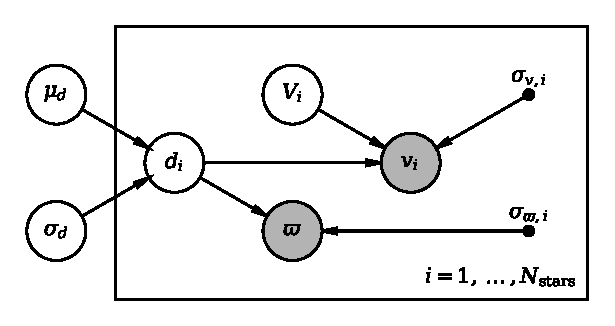
\includegraphics{figures/hbm-pgm.pdf}
    \caption[Probabilistic graphical model for the hierarchical model]{Probabilistic graphical model extension of Figure \ref{fig:simple-pgm} but for the HBM. The hyperparameters exist outside the box to show that they are the same across the population of stars.}
    \label{fig:hbm-pgm}
\end{figure}

We show the probabilistic graphical model of the HBM in Figure \ref{fig:hbm-pgm}. Here, we see how all individual stellar parameters depend on \(\mu_d\) and \(\sigma_d\). This is a simple extension of Figure \ref{fig:simple-pgm}, but with parameters existing outside the box to illustrate the model hierarchy. We can imagine extending this framework to multiple levels, or adding additional hyperparameters.

\subsection{Inferring the Model Parameters}\label{sec:hbm-inf}

To infer the model parameters, we need to calculate the marginalised posterior distributions for each parameter. We could obtain these analytically by integrating the full posterior distribution over all model parameters except for the parameter of interest. Alternatively, we can approximate the marginalised posterior using a Markov Chain Monte Carlo (MCMC) sampling algorithm. We chose the latter approach because it is scalable to more complicated models where the marginalisation is not analytically solvable.

To sample from the approximate posterior distribution for both models, we used the No U-Turn Sampler \citep[NUTS;][]{Hoffman.Gelman2014} as implemented in the \textsc{Python} package \texttt{numpyro} \citep{Phan.Pradhan.ea2019,Bingham.Chen.ea2019}. We ran the sampler for 1000 steps following 500 warm-up steps (used to adapt the sampling procedure) and repeated for 10 MCMC chains. To reduce the number of divergences encountered during sampling, we increased the target accept probability from 0.8 to 0.98 for the HBM. The resulting marginalised posterior samples amounted to \num{10000} per parameter.

\subsection{Comparing the Models}\label{sec:hbm-comp}

\begin{figure}[p]
    \centering
    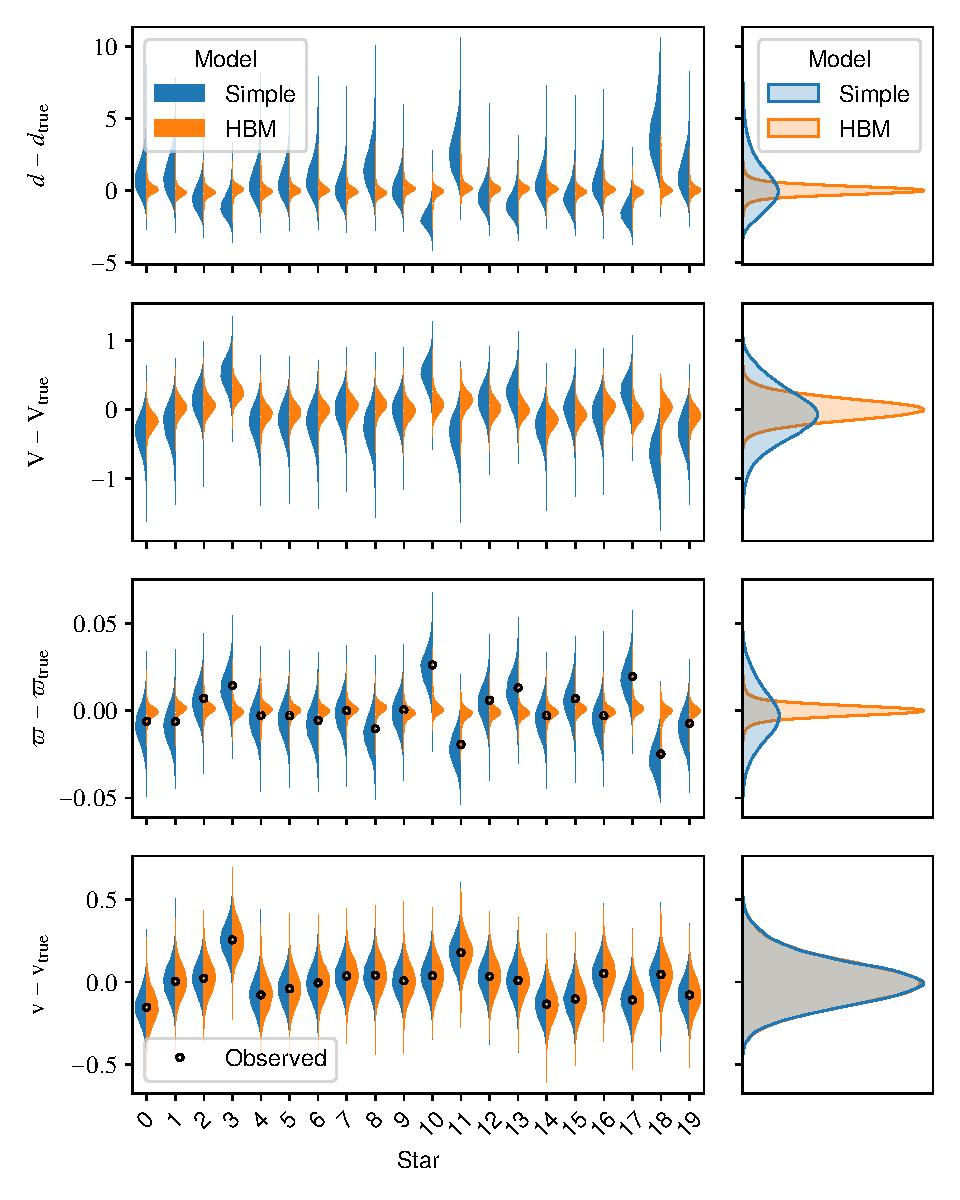
\includegraphics{figures/hbm-results.pdf}
    \caption[Plots comparing results from the simple model to the HBM]{Plots comparing results from the simple model (\emph{blue}) to the HBM (\emph{orange}). \emph{Left column:} Split violin-plots showing the difference between marginalised posterior distributions for the parameters and their true values. \emph{Right column:} Kernel density estimates of the parameter-truth differences over all \(N_\mathrm{stars}\). Observed values of the parameters are given by empty black circles.}
    \label{fig:hbm-results}
\end{figure}

We compared the difference between model parameters and their true values in Figure \ref{fig:hbm-results}. The HBM showed clear improvement over the simple model in all parameters except for apparent magnitude. Pooling the distances reduced their standard deviations by about one third and converged on their true values. This had the effect of reducing the observational noise on \(\varpi\), as we can see the posterior predictions for parallax also approached their true values. Since apparent magnitude depended on both \(d\) and \(\absmag\), better distances also improved the absolute magnitudes.

% \todo{Hand-wavy why apparent magnitude saw no improvement was because the observational noise on parallax had a larger impact on the distance than with apparent magnitude. \(\appmag \propto \log_{10}d\), whereas \(\varpi = d^{-1}\). Additionally, the fractional uncertainty on parallax was greater than that of apparent magnitude. The noise budget is dominated by the parallax, so this is the first to be improved by better distances. \(\sigma_\varpi/\varpi = \sigma_d \varpi\), but \(\sigma_\appmag / \appmag \propto \sigma_d \varpi / \appmag\)}

\begin{figure}
    \centering
    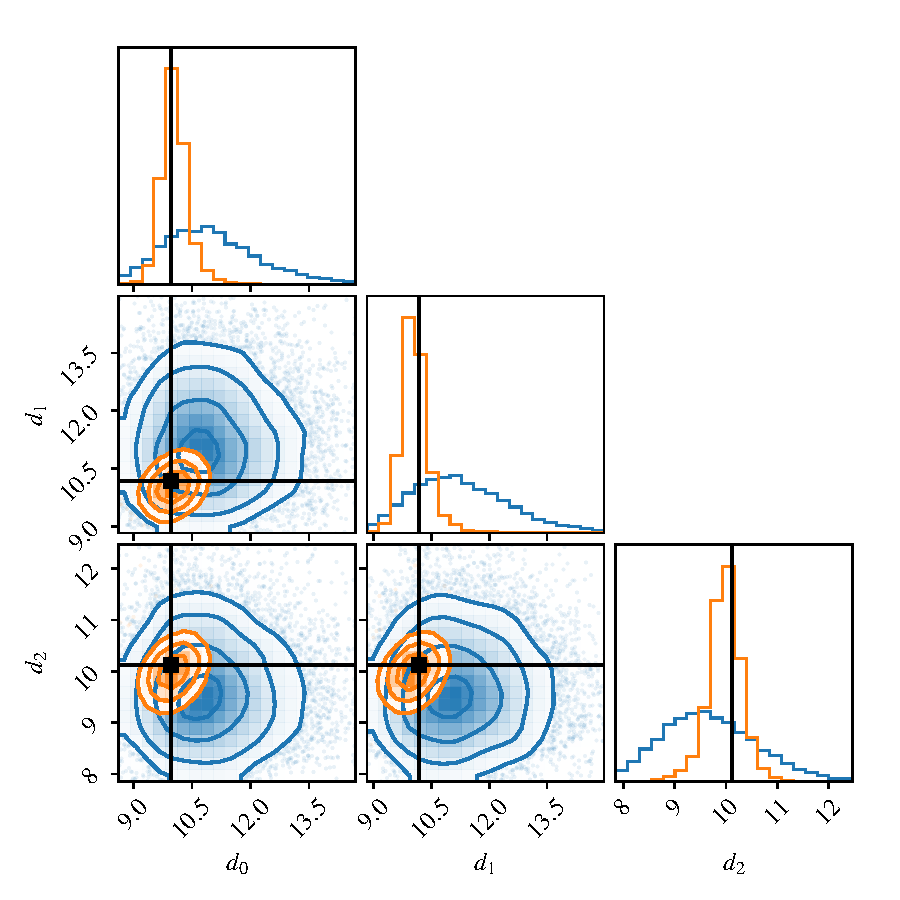
\includegraphics{figures/hbm-dist-corr.pdf}
    \caption[A corner plot showing the marginalised and joint posterior distributions of the distance to the first three stars]{A corner plot showing the marginalised and joint posterior distributions of the distance to the first three stars. The simple model is shown in \emph{blue} and the HMB is shown in \emph{orange}. The true values are given by the \emph{black} lines. The range of the distributions are limited to 98 per cent of the simple model's marginalised posteriors.}
    \label{fig:hbm-corr}
\end{figure}

In Figure \ref{fig:hbm-corr}, we compared the joint and marginalised posteriors of the distance to a few of the stars. The HBM found distances to higher precision, with typical standard deviations of \(s_{d,i} \approx 0.35\) compared to \(s_{d,i} \approx 1.2\) from the simple model. We also noticed a one-to-one correlation between \(d\) present in the HBM but not in the simple model. This was a result of the correlation introduction by the population-prior on \(d\). For each distance, we saw how a lower value in one corresponded to a lower value for the others. This represents our belief that cluster members should share a similar distance. On the other hand, the simple model suggested it was, for example, just as likely to find two stars at distances of 9 and 12 as it would for both to be at a distance of 11.

\begin{figure}[tb]
    \centering
    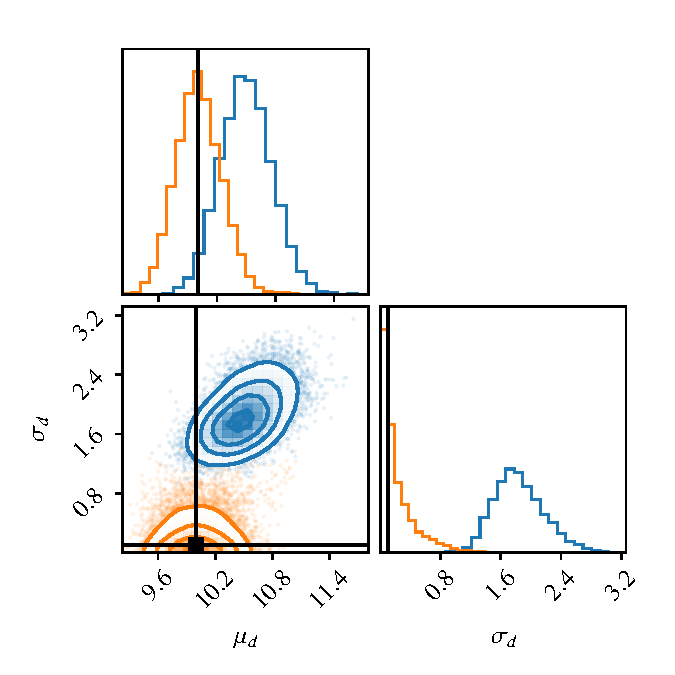
\includegraphics{figures/hbm-global.pdf}
    \caption[The joint and marginalised posterior distributions for the mean and standard deviation of stellar distances in the cluster]{The joint and marginalised posterior distributions for the mean (\(\mu_d\)) and standard deviation (\(\sigma_d\)) of stellar distances in the cluster. The simple model is shown in \emph{blue} and the HMB is shown in \emph{orange}. The true values are given by the \emph{black} lines.}
    \label{fig:hbm-global}
\end{figure}

One consequence of the HBM was that it parametrised the population mean (\(\mu_d\)) and standard deviation (\(\sigma_d\)) of the distances to stars in the cluster separately from the observed noise. For the simple model, we estimated \(\mu_d\) and \(\sigma_d\) by taking the sample mean and standard deviation of distances in the cluster for each posterior sample. We compared the resulting posterior distributions for \(\mu_d\) and \(\sigma_d\) from the two models in Figure \ref{fig:hbm-global}. The mean distance from the simple model was \(\mu_d = 10.50 \pm 0.27\), whereas the HBM was more accurate with \(\mu_d = 10.01 \pm 0.24\). The simple model massively overestimated the standard deviation of cluster distances with \(\sigma_d = 1.815_{-0.293}^{+0.360}\), compared to the HBM's more accurate value of \(\sigma_d = 0.131_{-0.088}^{+0.280}\). The simple model could not distinguish between the uncertainty on individual distances and the spread of the population.

\subsection{Scaling with the Number of Stars}\label{sec:hbm-scale}

To test how the model scales with number of stars, we repeated the HBM method for different \(N_\mathrm{stars}\). We randomly generated true and observed parameters in the same way as described at the beginning of \ref{sec:hbm-dist} for 320 stars. The observables were different to the last section, but drawn from the same distributions. We then sampled from the HBM for the first 20, 80 and 320 stars. These represented ratios in \(N_\mathrm{stars}^{1/2}\) of \(1\), \(2\) and \(4\) respectively.

\begin{figure}[tb]
    \centering
    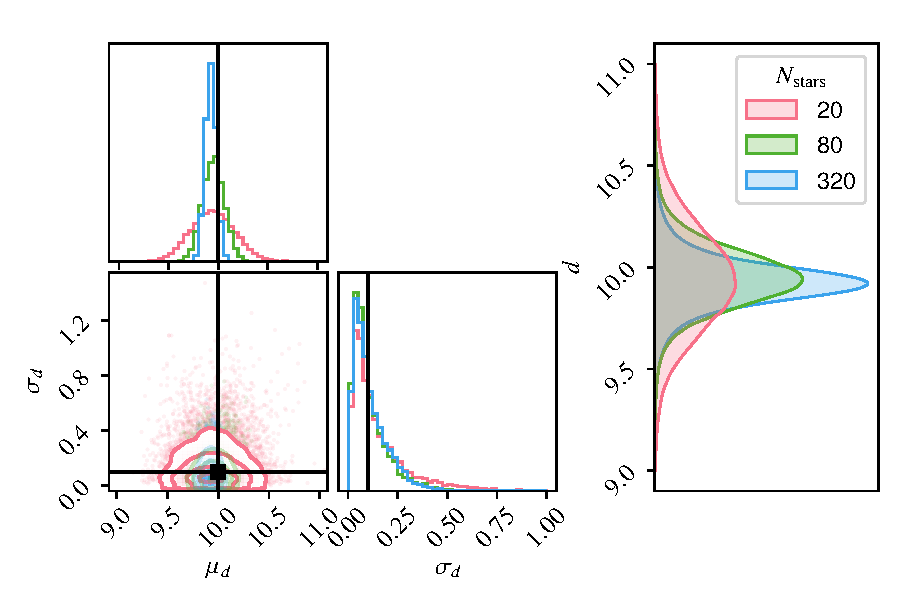
\includegraphics{figures/hbm-extended.pdf}
    \caption{Joint and marginalised posterior distributions from the HBM for 20, 80 and 320 stars.}
    \label{fig:hbm-extended}
\end{figure}

Figure \ref{fig:hbm-extended} shows how the distance estimates improved with increasing number of stars observed, \(N_\mathrm{stars}=(20,80,320)\). Unsurprisingly, the standard deviation on \(\mu_d\) decreased by a factor of \(N_\mathrm{stars}^{1/2}\) each time, with \(s_{\mu_d} \approx (0.24, 0.12, 0.06)\). We also expected a similar reduction in uncertainty for individual distances, albeit limited by the observational noise. Typical standard deviations for \(d_i\) were \(s_{d,i} \approx (0.30, 0.17, 0.15)\). As expected, the distance uncertainties also halved from \(20\) to \(80\) stars. However, this effect lessened with 320 stars. This demonstrated the method is still limited by the error budget across all observed parameters. Despite this, the HBM proved to be a useful way of getting more information from a limited number of noisy observations. 

\section[Stellar Properties]{Inferring Physical Properties of Stars}\label{sec:hbm-phys}

We have seen how a simple HBM can be used to improve the distances and absolute magnitudes of stars in a cluster analogue. This kind of model only represents part of the puzzle for determining ages, masses, and radii in a population of stars. In these Bayesian stellar models (discussed previously in Section \ref{sec:modelling-stars}) we have more parameters which could be considered hierarchically. In this section, we discuss a few possible population distributions which could form a hierarchical model of stellar physics.

\paragraph{Mass} As mentioned in the introduction to this chapter, an IMF may be used as a prior on the mass of a star. If modelling stars with masses spanning a couple of orders of magnitude, it makes sense to draw their masses from an IMF. To make this hierarchical, we would parametrise the IMF as a conditional distribution which informs individual stellar masses. This way, the population of stars constrains the IMF while in-turn sharing information. In this thesis, we only consider stars in a narrow mass range (\SIrange{0.8}{1.2}{\solarmass}) where the IMF does not change much. However, a mass hierarchy like this may be useful in future work.

\paragraph{Age} We do not expect a star to be older than the universe. This makes the age of the universe a natural upper limit to a prior on stellar age. There are also populations of stars where we expect the age to be tightly related. For example, star systems like binaries and clusters are expected to have been formed at a similar time. Similarly to the distances in Section \ref{sec:hbm-dist}, a hierarchical model in age would parametrise the mean and variance of ages in these systems and in-turn improve other connected model parameters. This sort of analysis could be extended to find mixtures of age distributions in the galaxy which could indicate mergers \citep[e.g. \emph{Gaia}-Enceladus;][]{Helmi.Babusiaux.ea2018}. However, we do not further consider an HBM in age this in this work.

\paragraph{Chemical Abundances} Unlike mass and age, surface abundances of stars can be measured directly with spectroscopy. However, not all abundances are easily measured. For example, helium ionises below the surface of the cool stars being studied in this work. Also, diffusion and settling of elements during stellar evolution means surface abundances differ from formation to time of observation. Similarly to age, we can expect clusters of stars to share initial abundances. However, the distribution of abundances in the Milky Way may also be parametrised. As stars evolve they convert hydrogen into helium and heavier elements. Supernovae enrich the galaxy with these elements monotonically, which go on to constitute new stars. A hierarchical model could include this assumption to tie the abundance of helium to heavier elements.

\paragraph{Approximations of Stellar Physics} A hierarchical model need not be limited to real physical parameters. In stellar modelling, we often approximate stellar physics with \emph{pseudo}-physical parameters. For example, convective energy transfer is approximated by the mixing-length theory \citep[MLT;][]{Gough1977} parametrised by \(\mlt\). The value of \(\mlt\) which best models a star is likely to vary with other stellar parameters. It's effect on observables is small making \(\mlt\) difficult to constrain on a star-by-star basis. Hence, a hierarchical model would be able to condition individual values of \(\mlt\) on its population distribution. A distribution over pseudo-physical parameters is less intuitive, yet the HBM would allow us to build one empirically. In addition to the initial helium abundance, \(\mlt\) is modelled hierarchically in Chapter \ref{chap:hmd}.
